% Created 2022-12-15 Thu 18:45
% Intended LaTeX compiler: pdflatex
\documentclass[presentation]{beamer}
\usepackage{amsmath}
\usepackage[utf8]{inputenc}
\usepackage[T1]{fontenc}
\usepackage{graphicx}
\usepackage{longtable}
\usepackage{wrapfig}
\usepackage{rotating}
\usepackage[normalem]{ulem}
\usepackage{amsmath}
\usepackage{amssymb}
\usepackage{capt-of}
\usepackage{hyperref}
\usepackage{listings}
\newcommand{\labelitemi}{$\bullet$}
\newcommand{\labelitemii}{$\circ$}
\usepackage{enumitem}
\usepackage{helvet}
\lstdefinelanguage{yaml}{basicstyle=\ttfamily\tiny,frame=tblr,framerule=.2pt,framexleftmargin=1pt,showstringspaces=false,escapechar=\@}
\lstdefinelanguage{sh}{basicstyle=\ttfamily\tiny,frame=tblr,framerule=.2pt,framexleftmargin=1pt,showstringspaces=false,escapechar=\@}
\usetheme{Madrid}
\author{Petra Kalocsai, Tamás Lévai, Gábor Rétvári (BME)}
\date{}
\title{A Multi-cluster SD-WAN East-west Gateway}
\setbeamertemplate{items}[circle]
\hypersetup{
 pdfauthor={Petra Kalocsai, Tamás Lévai, Gábor Rétvári (BME)},
 pdftitle={A Multi-cluster SD-WAN East-west Gateway},
 pdfkeywords={},
 pdfsubject={},
 pdfcreator={Emacs 27.1 (Org mode 9.5.2)}, 
 pdflang={English}}
\begin{document}

\maketitle

\begin{frame}[label={sec:orge356828}]{Goals}
\begin{itemize}
\item build an \alert{east-west (EW) gateway} to seamlessly \alert{interconnect two or more service-mesh clusters
over an SD-WAN fabric} for a consistent end-to-end user experience
\item integrate the \alert{L4/L7 traffic management policies} on the service-mesh side with the \alert{L3/L4
policies} on the SD-WAN interconnect
\item end-to-end \alert{observability and the security} across the service mesh and the SD-WAN segments
\item demos!
\end{itemize}

\begin{center}
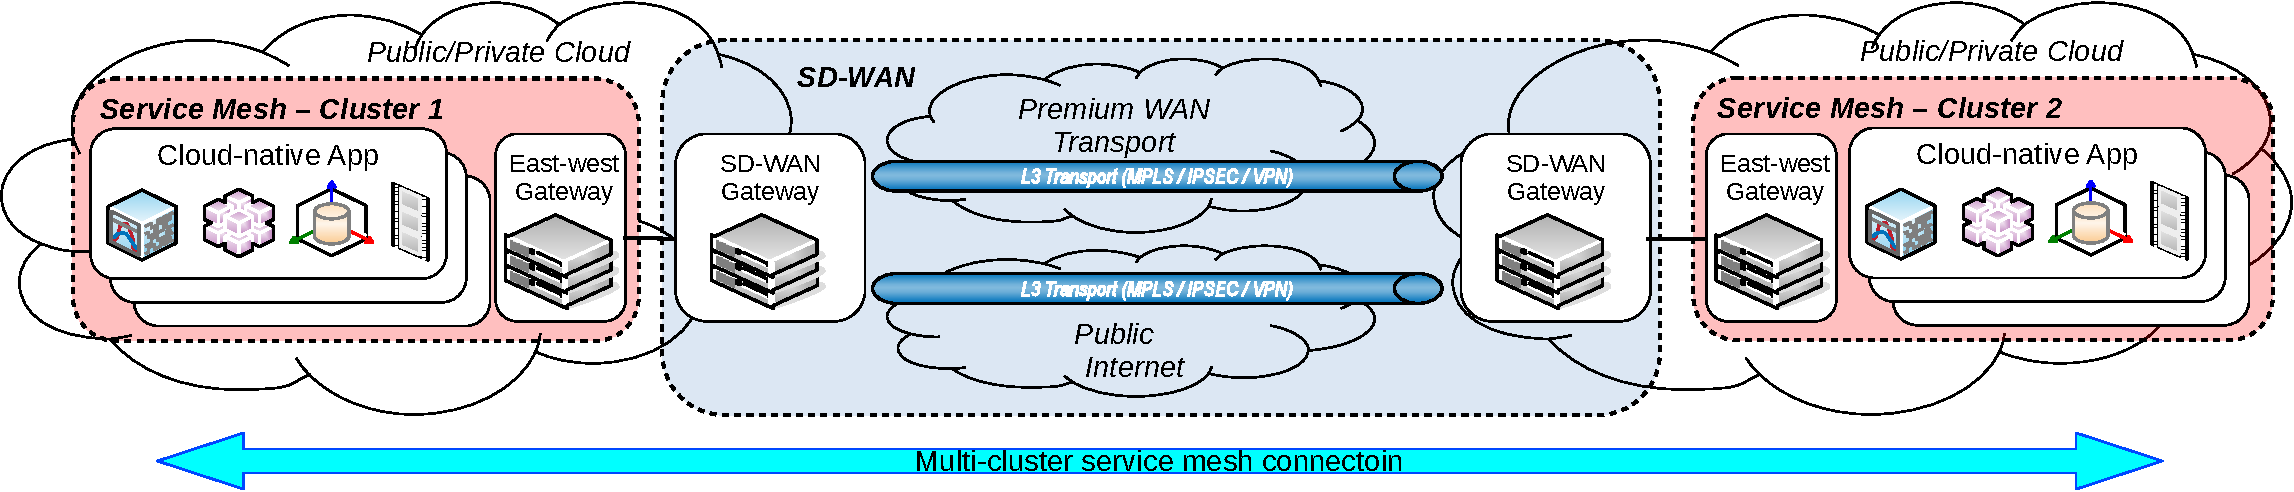
\includegraphics[width=340pt]{./multi-cluster-service-mesh-ew-gateway-reference-arch-crop.pdf}
\end{center}
\end{frame}

\begin{frame}[label={sec:org7aa4b00},fragile]{User stories}
 \begin{itemize}
\item \alert{service-level SD-WAN policies:} the service owner wants all accesses to the \texttt{payment.secure} HTTP
service (port 8080) to be mapped to the high-prio SD-WAN tunnel
\item \alert{L7 traffic management:} same, but now only GET queries to the API endpoint \texttt{/payment} should map
to the high-prio tunnel
\item \alert{resiliency:} automatic failover between SD-WAN tunnels
\item \alert{monitoring:} end-to-end observability
\end{itemize}
\end{frame}

\begin{frame}[label={sec:org1f54e76}]{Principles}
\begin{itemize}
\item \alert{\alert{separate traffic flows intended to be sent over different SD-WAN tunnels}} on the egress EW
gateway, in order for the SD-WAN to be able to apply the proper SD-WAN priority
\item services between clusters are exported/imported using the
\href{https://gateway-api.sigs.k8s.io}{\alert{\alert{Multi-cluster Services API (KEP-1645) CRDs}}}, extended
with a set of annotations to control SD-WAN routing policies
\item \alert{L7 policies can be applied on top of the service-level exports/imports} to control the way
traffic egresses from, and ingresses into, the cluster
\end{itemize}
\end{frame}

\begin{frame}[label={sec:org727b29f}]{Service-level traffic management}
\begin{itemize}
\item \alert{associate an SD-WAN policy with distinct Kubernetes service}
\item no way to impose additional L7-level SD-WAN policies on top (yet)
\item basic model will be extended to a fully-fledged L7 model later
\item separate CRDs to define WAN policies, service exports and service imports
\end{itemize}
\end{frame}

\begin{frame}[label={sec:orge5faad5},fragile]{WAN policies}
 \begin{itemize}
\item each global service can have a WAN policy associated with it, defined in a cluster-global CRD
named \texttt{WANPolicy.mcw.l7mp.io}
\item format is unspecified for now; below is a sample to define 2 policies
\begin{itemize}
\item \alert{high-priority tunnel} with stringent SLAs associated with the port 31111
\item \alert{high-priority tunnel} with less stringent SLAs associated with the port 31112
\end{itemize}
\lstset{language=yaml,label= ,caption= ,captionpos=b,numbers=none}
\begin{lstlisting}
apiVersion: mcw.l7mp.io/v1alpha1
kind: WANPolicy
metadata:
name: sd-wan-priority-high
spec:
  tunnel: business
  port: 31111
  sla:
    jitter-ms: 50
    latency-ms: 100
    loss-percent: 1
\end{lstlisting}
\end{itemize}
\end{frame}

\begin{frame}[label={sec:org4159600},fragile]{Service exports}
 \begin{itemize}
\item services have to be explicitly exported from the hosting cluster to allow access from other
clusters
\item the below will export the service called \texttt{payment} in the \texttt{secure} namespace over the high-prio
SD-WAN tunnel
\lstset{language=yaml,label= ,caption= ,captionpos=b,numbers=none}
\begin{lstlisting}
apiVersion: multicluster.k8s.io/v1alpha1
kind: ServiceExport
metadata:
  name: payment
  namespace: secure
  annotations:
    mcw.l7mp.io/mc-wan-policy: sd-wan-priority-high
\end{lstlisting}
\end{itemize}
\end{frame}

\begin{frame}[label={sec:org6577dd6},fragile]{Service imports}
 \begin{itemize}
\item exported services are automatically imported into all clusters in which the service's namespace
exists (including the exporting cluster)
\item ServiceImport CRDs are automatically created by the controller
\lstset{language=yaml,label= ,caption= ,captionpos=b,numbers=none}
\begin{lstlisting}
apiVersion: multicluster.k8s.io/v1alpha1
kind: ServiceImport
metadata:
  name: payment
  namespace: secure
spec:
  type: ClusterSetIP
  ports:
  - name: http
    protocol: TCP
    port: 8080
\end{lstlisting}
\end{itemize}
\end{frame}

\begin{frame}[label={sec:orgb2630b0}]{Demo!}
\end{frame}

\begin{frame}[label={sec:org15e3e38},fragile]{L7 traffic management}
 \begin{itemize}
\item up to this point, SD-WAN policies could be applied to individual Kubernetes services only
\item the below shows how to add L7 traffic management policies by reusing the
ServiceImport/ServiceExport CRs
\item we assume that the \texttt{payment.secure} service is exported over both the high- (\texttt{payment-high-prio})
and the low-priority tunnel (\texttt{payment-low-prio})
\end{itemize}
\end{frame}

\begin{frame}[label={sec:org78a4d23},fragile]{Client-side L7 HTTP request routing}
 \begin{itemize}
\item goal is to route requests to different SD-WAN tunnels depending on the HTTP headers
\item in the below, only GET requests to the \texttt{/payment} HTTP path would be routed to the high-priority
tunnel, everything else should go over low-prio tunnel
\lstset{language=yaml,label= ,caption= ,captionpos=b,numbers=none}
\begin{lstlisting}
apiVersion: networking.istio.io/v1beta1
kind: VirtualService
metadata:
  name: payment
  namespace: secure
spec:
  hosts:
  - payment.secure.svc.clusterset.local
  http:
  - match: [ uri: {prefix: "/payment" }, method: { exact: GET } ]
    route:
    - destination:
        host: payment-high-prio.secure.svc.clusterset.local
  - route:
    - destination:
        host: payment-low-prio.secure.svc.clusterset.local
\end{lstlisting}
\end{itemize}
\end{frame}

\begin{frame}[label={sec:org6f16264}]{Demo!}
\end{frame}

\begin{frame}[label={sec:orgd2cbe97},fragile]{Command line tool (WiP!)}
 \begin{itemize}
\item there is a proof-of-concept command line tool to automate service imports and service exports
\lstset{language=sh,label= ,caption= ,captionpos=b,numbers=none}
\begin{lstlisting}
# export a service
mcwanctl --context $CTX1 export payment/secure --wan-policy=high
# get status
mcwanctl --context $CTX1 status payment/secure
# import 
mcwanctl --context $CTX2 import payment/secure --ingress-gw=<GW_IP_ADDRESS>
\end{lstlisting}
\item ingress Gateways already done
\item Petra is working on it!
\end{itemize}
\end{frame}

\begin{frame}[label={sec:org582e42f},fragile]{Further plans}
 \begin{itemize}
\item play with the \alert{\alert{spec}}, see pros and cons in practice
\item find new ways to \alert{\alert{map the semantics to existing Kubernetes APIs}}
\item implement the \alert{\alert{command line tool}}
\item implement a \alert{\alert{fully-fledged multi-cluster API operator}} to automatically reconcile
ServiceImports/ServiceExports
\item integrate with the \alert{\alert{\texttt{l7mp/stunner} Kubernetes Gateway project}}
\end{itemize}
\end{frame}
\end{document}
